%!TEX root = ../summary.tex

\section{From Source Code to Physical Deployment}

\subsection{Version Control Systems}
Versioning aims to control an manage all artifacts used and created in a process.
VCSes can be differentiated between local, centralized and distributed VCSes.
Local ones are kept only on the local systems where the artifacts are developed.
Centralized VCSes have a central server that holds the code base and single clients have only a single version of the artifacts available.
Distributed VCSes have different versions locally as well as on a central repository.

\subsubsection{SVN (central) vs Git (distributed)}
SVN stores information as a list of file-based changes.
Git on the other hand handles the data more like a set of snapshots of a miniature file system.
Every commit is a picture taken of what all files look like at that moment and pointers to these snapshots are stored.

\subsubsection{Git}
\paragraph{File States}
In Git, a file can have three different stages.
In the modified state the file has changes that are not yet committed to the local database.
In the staged state the file then has been marked to go into the next commit and in the committed state the data is safely stored in the local database.
In that state the data can be pushed to the remote repository.

\paragraph{Commands}
\begin{figure}[H]
  \centering
  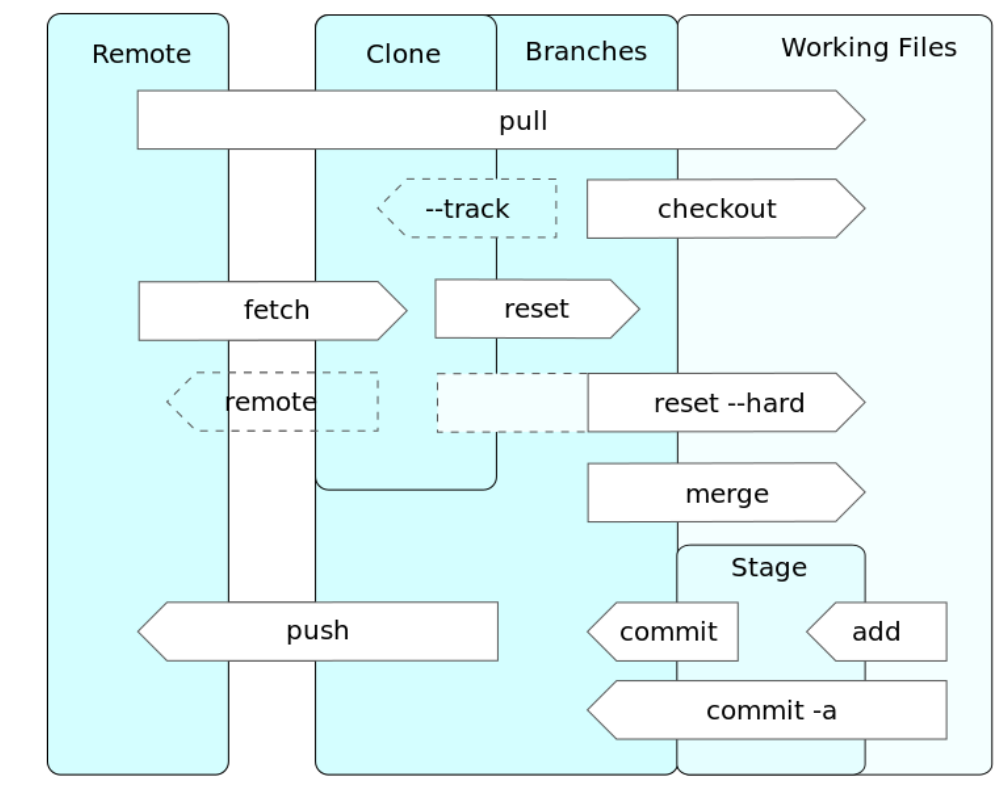
\includegraphics[width=.8\textwidth]{images/git_commands.png}
  \caption{Git Commands}
\end{figure}

\paragraph{Branching}
Git keeps snapshots of the commits named by hashes of the local files.
Branches are pointers to these commits.
The HEAD pointer points to the current local commit, the default branch is called master and adding a branch means adding a named pointer to a commit.

\subsection{Continuous Integration}
\begin{figure}[h]
  \centering
  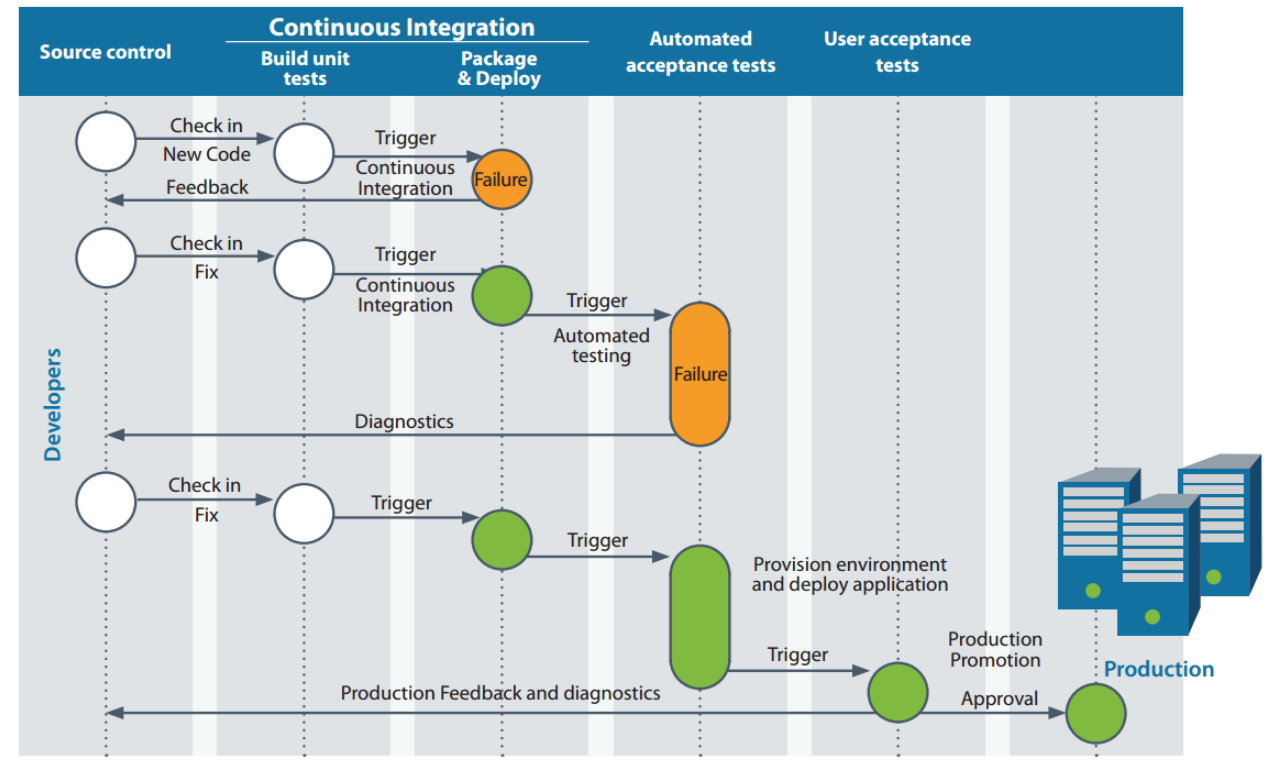
\includegraphics[width=.8\textwidth]{images/continuous_integration.png}
  \caption{Continuous Integration}\label{fig:continuous_integration}
\end{figure}
A development process (c.f.\ Figure~\ref{fig:continuous_integration}) with continuous integrations maintains a single source repository with an automated build and tests.
Every commit triggers a this automated procedures for what it is important to keep the build process fast.
Test should be executed in a clone of the production environment.
The automated build process makes it easy for everyone to get the latest executables and makes the result visible to everyone.
In the end, even the deployment can be automated potentially.\\

\textbf{Pros}
\begin{itemize}[topsep=0pt, noitemsep]
  \item Reducing risk
  \item Integrated quality assurance
  \item Reports and feedback on the health of the code base
  \item Availability of a stable release
  \item Everyone commits to the main branch every day which results in modular, less complex code
\end{itemize}

\subsection{Continuous Deployment}
Continuous deployment means that every change goes through the pipeline and automatically gets put into production, resulting in many production deployments every day.
For continuous deployment continuous delivery is necessary.
This is a software engineering approach in which teams keep producing valuable software in short cycles and ensure that the software can be reliably released at any time.\\

A deployment pipeline is essential for automating the deployment process.
It represents an automated manifestation of the process of getting software from version control into the hands of the users.
It builds binaries deploys them the same way in every environment after some ``smoke-tests''.
If it fails at any point, the deployment process is stopped.

\paragraph{Deployment-automation Patterns}
\begin{figure}[H]
  \centering
  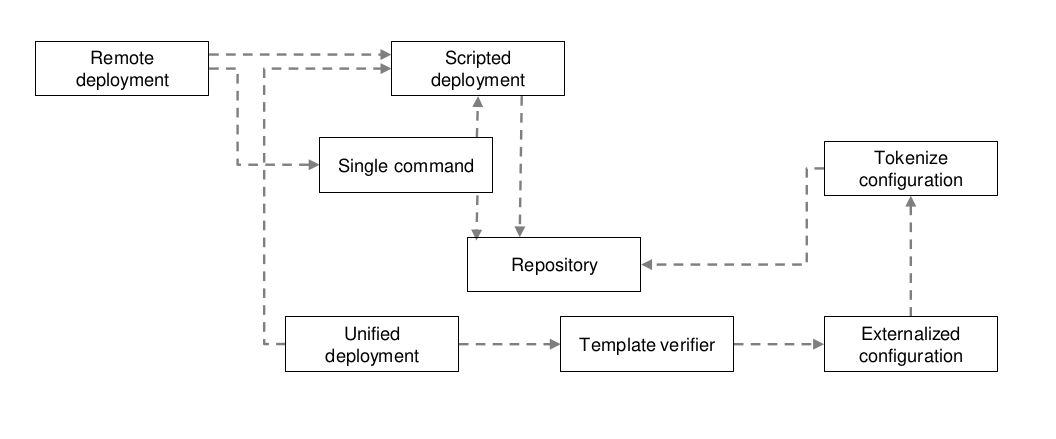
\includegraphics[width=.8\textwidth]{images/deployment_automation_patterns.png}
  \caption{Deployment-automation Patterns}
\end{figure}
\begin{description}
  \item[Repository] All files are committed to version-control repository — in the deployment context, all of the configuration files and tools.
  \item[Scripted deployment] All deployment processes are written in a script.
  \item[Single command] Deployers, or headless processes, can type a single command to generate working software for users.
  \item[Externalized configuration] All variable values are externalized from the application configuration into build-time properties.
  \item[Tokenize configuration] Token values are entered into configuration files and then replaced during the Scripted Deployment based on Externalized Configuration properties checked into Repository.
  \item[Template verifier] Create a single template file that all target environment properties are based on.
  \item[Unified deployment] Create a single deployment script capable of running on different platforms and target environments.
  \item[Remote deployment] Use a centralized machine or cluster to deploy software to multiple target environments.
\end{description}

\paragraph{Blue Green Deployment}
In blue green deployment, two different production environments are maintained.
In the start the blue one is live.
For a new release, perform a final stage of testing in the green environment and once the software is working, switch to green.

\subsection{Virtual Machines and Containers}
\paragraph{Virtualization}
Virtualization is a combination of software and hardware engineering that creates Virtual Machines (VMs) - an abstraction of the computer hardware that allows a single machine to act as if it where many machines.
This enables the current model of data centers where many virtual machines run on one machine.

\paragraph{Containers}
Containers apply virtualization at the operating system level instead of the hardware level (c.f.\ Figure~\ref{fig:container_vs_virtual_machines}).
This makes containers smaller than hypervisor guests but does not allow running different kernels and has a more loosely approach to isolation and security.\\
\begin{figure}[h]
  \centering
  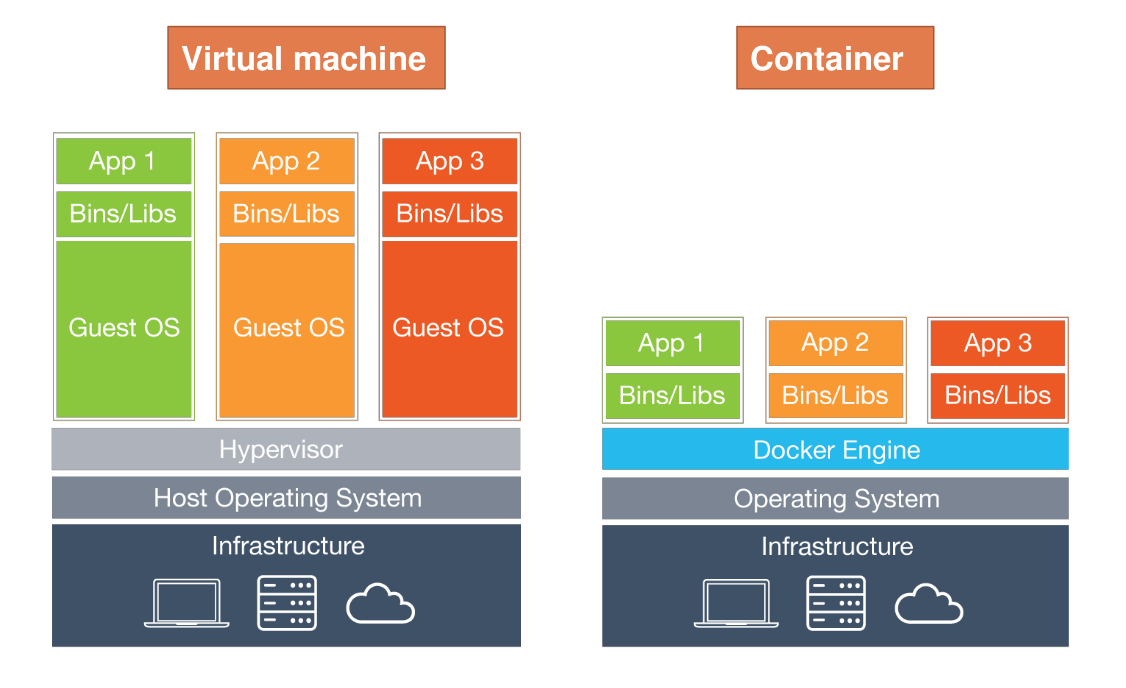
\includegraphics[width=.8\textwidth]{images/container_vs_virtual_machines.png}
  \caption{Virtual Machines vs Application Containers}\label{fig:container_vs_virtual_machines}
\end{figure}

The most popular system for container virtualization is Docker.
Its system is depicted in Figure~\ref{fig:docker}.
\begin{figure}[H]
  \centering
  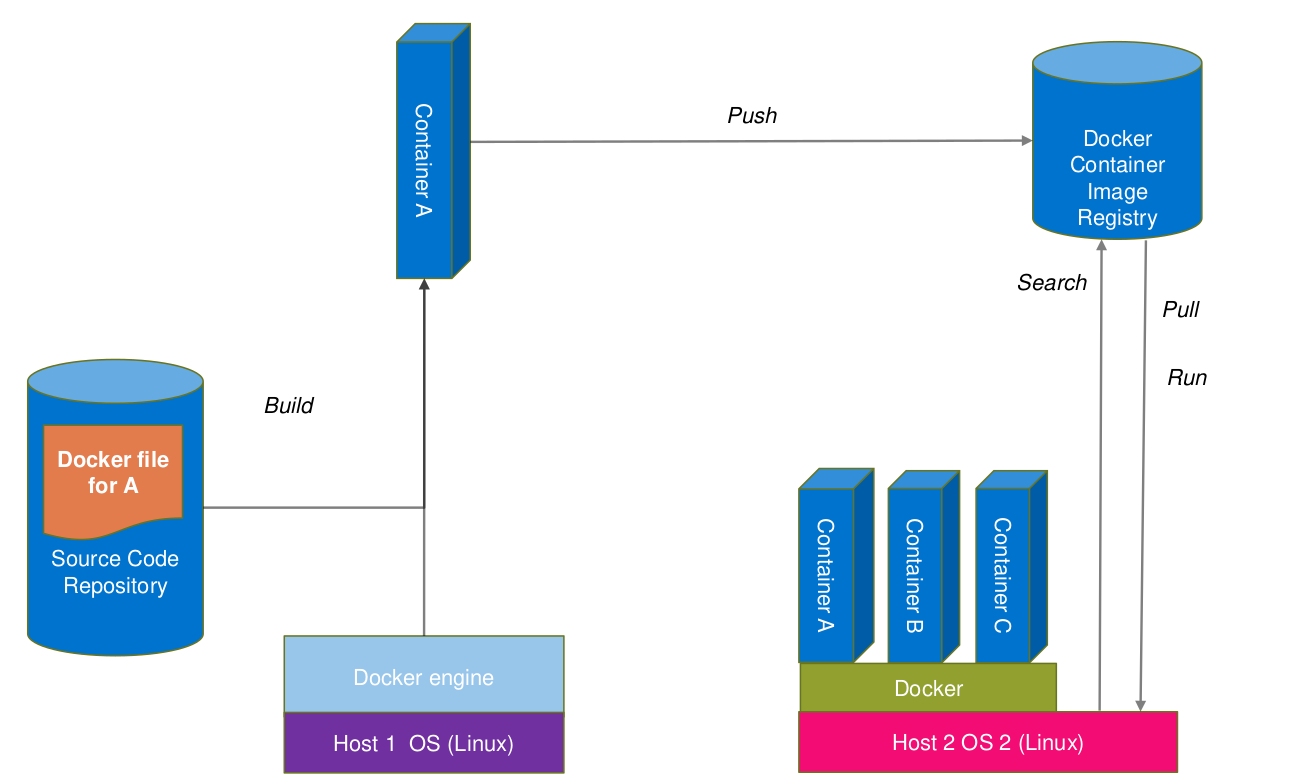
\includegraphics[width=.8\textwidth]{images/docker.png}
  \caption{Docker System}\label{fig:docker}
\end{figure}

\subsection{Software Architecture for the cloud}
The cloud is a style of computing in which scalable and elastic IT-enabled capabilities are delivered as a service to external customers using Internet technologies.\\
The main goals are increased availability and reachability, reduced investments and increased stability.
The main challenges are confidentiality, integrity, availability, privacy, the increased attack surface it implies, the difficulty to audit the system, as well as legal and trust issues.\\
The cloud provides on-demand self-service, broad network access and resource pooling.

\paragraph{Cloud Reference Architecture}
\begin{figure}[H]
  \centering
  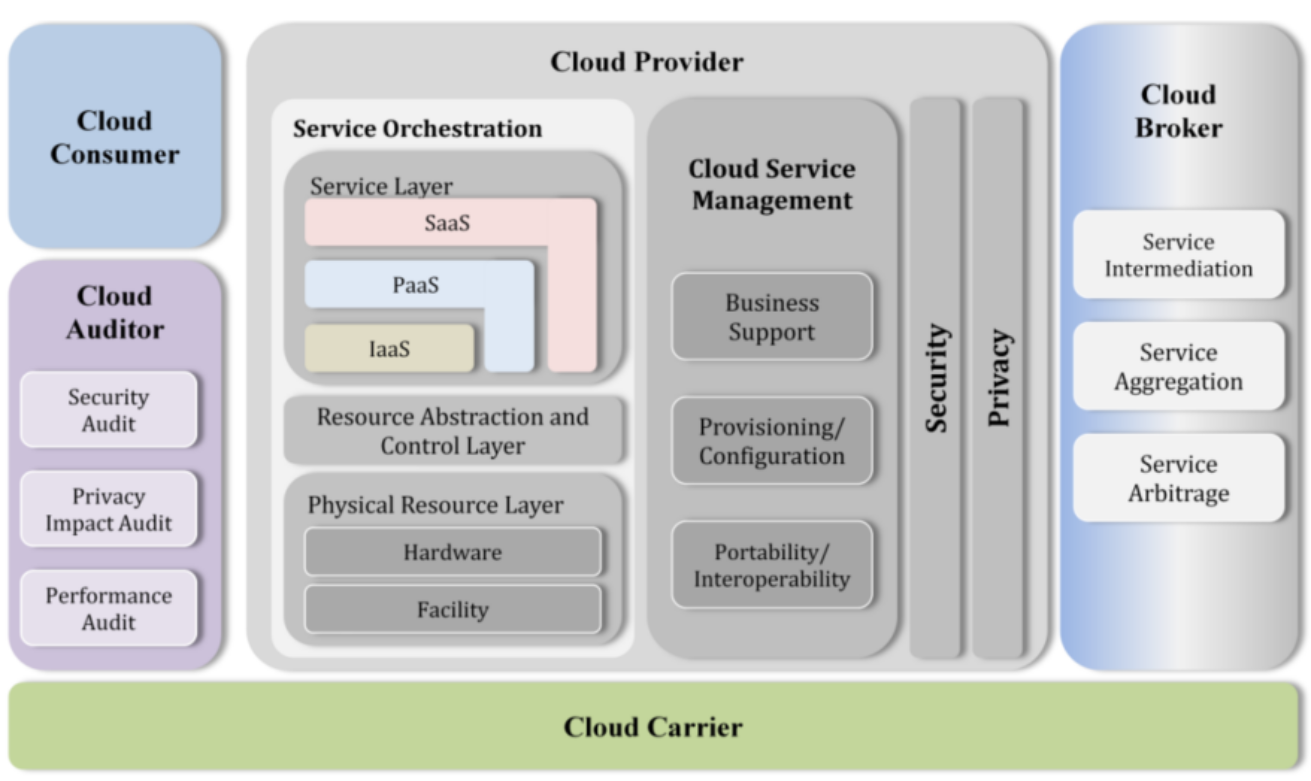
\includegraphics[width=.8\textwidth]{images/cloud_reference_architecture.png}
  \caption{Cloud Reference Architecture}
\end{figure}
\begin{description}
  \item[Cloud consumer] A person or organization that maintains a business relationship with, and uses service from, cloud providers.
  \item[Cloud provider] A person, organization, or entity responsible for making a service available to interested parties.
  \item[Cloud auditor] A party that can conduct independent assessment of cloud services, information system operations, performance and security of the cloud implementation.
  \item[Cloud broker] An entity that manages the use, performance and delivery of cloud services, and negotiates relationships between cloud providers and cloud consumers.
  \item[Cloud carrier] An intermediary that provides connectivity and transport of cloud services from cloud providers to cloud consumers.
\end{description}

\paragraph{Xaas}
\textbf{Software as a Service (Saas)} provides applications running on the cloud to consumers.
Network, Severs, OS and Storage is all handled by the provider, the consumer interacts with the cloud through client interfaces as a web browser or a program interface. (Google Apps, Dropbox, Office 365)\\

\textbf{Platform as a Service (PaaS)} provides the consumer with programming languages,
libraries, services, and tools who is then able to deploy an application into that environment.
The provider still handles network, servers, OS and storage but the consumer has control over the deployed applications. (Github, Google App Engine)\\

\textbf{Infrastructure as a Service (IaaS)} provides the consumer with processing, storage, network and other fundamental computing resources onto which the customer can deploy arbitrary software (including OSes).
The consumer here as control over OS, storage, deployed applications and a limited set of network components like firewalls.(Amazon Web Services, Google Compute Engine, Microsoft Azure)

\paragraph{Deployment Model}
A \textbf{public cloud infrastructure} is provisioned for open use by the general public.
It may be owned, managed, and operated by a business, academic, or government organization, or some combination of them.
It exists on the premises of the cloud provider.\\

In a \textbf{private and out-sourced private cloud}, the infrastructure is provisioned for exclusive use by a single organization comprising multiple consumers (e.g.\ business units).
It may be owned, managed, and operated by the organization, a third party, or some combination of them, and it may exist on or off premises.\\

A \textbf{community cloud infrastructure} is provisioned for exclusive use by a specific community of consumers from organizations that have shared concerns (e.g.\ mission, security requirements, policy, and compliance considerations).
It may be owned, managed, and operated by one or more of the organizations in the community, a third party, or some combination of them, and it may exist on or off premises.\\

In a \textbf{hybrid model} the cloud infrastructure is a composition of two or more distinct cloud infrastructures (private, community, or public) that remain unique entities, but are bound together by standardized or proprietary technology that enables data and application portability (e.g.\ cloud bursting for load balancing between clouds).

\paragraph{Fundamental Cloud Architectures}
In a \textbf{workload distribution architecture} IT resources can be horizontally scaled via the addition of one or more identical IT resources, and a load balancer that provides runtime logic capable of evenly distributing the workload among the available IT resources.\\

A special version of this is the \textbf{service load balancing architecture} which is geared specifically for scaling cloud service implementations.
Redundant deployments of cloud services are created, with a load balancing system added to dynamically distribute workloads.\\

A \textbf{resource pooling architecture} is based on the use of one or more resource pools, in which identical IT resources are grouped and maintained by a system that automatically ensures that they remain synchronized.\\

The \textbf{dynamic scalability architecture} is an architectural model based on a system of predefined scaling conditions that trigger the dynamic allocation of IT resources from resource pools.
Dynamic allocation enables variable utilization as dictated by usage demand fluctuations.
This scaling can happen horizontally by adding new instances or vertically by increasing the resources of a single instance.
An hybrid approach is also possible.\\
